\section*{Data Models}
\begin{frame}[fragile]{\texttt{src/emergency\_planner/data\_models/}}
  \begin{columns}[c]
    \begin{column}{0.3\textwidth}
        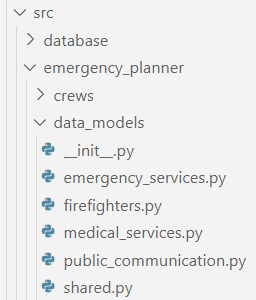
\includegraphics[width=\textwidth]{figures/data_models_folder.png}
    \end{column}
    \begin{column}{0.68\textwidth}
      \texttt{shared.py}
      \begin{lstlisting}[language=Python, breaklines=true]
FireType = Literal["ordinary",..., "other"]
FireSeverity = Literal["low", "medium", "high"]
... 
def add_schema_to_task_config(task_config, schema):
   ...
    return task_config
      \end{lstlisting}
      \texttt{public\_communication.py}
      \begin{lstlisting}[language=Python, breaklines=true]
from pydantic import BaseModel
from .shared import FireSeverity, FireType
from .medical_services import MedicalResponseReport
...
class EmergencyReport(BaseModel):
  medical_response_report: MedicalResponseReport
  fire_type: FireType
  fire_severity: FireSeverity
  ...
      \end{lstlisting}
    \end{column}
  \end{columns}
\end{frame}